\documentclass[1p]{elsarticle_modified}
%\bibliographystyle{elsarticle-num}

%\usepackage[colorlinks]{hyperref}
%\usepackage{abbrmath_seonhwa} %\Abb, \Ascr, \Acal ,\Abf, \Afrak
\usepackage{amsfonts}
\usepackage{amssymb}
\usepackage{amsmath}
\usepackage{amsthm}
\usepackage{scalefnt}
\usepackage{amsbsy}
\usepackage{kotex}
\usepackage{caption}
\usepackage{subfig}
\usepackage{color}
\usepackage{graphicx}
\usepackage{xcolor} %% white, black, red, green, blue, cyan, magenta, yellow
\usepackage{float}
\usepackage{setspace}
\usepackage{hyperref}

\usepackage{tikz}
\usetikzlibrary{arrows}

\usepackage{multirow}
\usepackage{array} % fixed length table
\usepackage{hhline}

%%%%%%%%%%%%%%%%%%%%%
\makeatletter
\renewcommand*\env@matrix[1][\arraystretch]{%
	\edef\arraystretch{#1}%
	\hskip -\arraycolsep
	\let\@ifnextchar\new@ifnextchar
	\array{*\c@MaxMatrixCols c}}
\makeatother %https://tex.stackexchange.com/questions/14071/how-can-i-increase-the-line-spacing-in-a-matrix
%%%%%%%%%%%%%%%

\usepackage[normalem]{ulem}

\newcommand{\msout}[1]{\ifmmode\text{\sout{\ensuremath{#1}}}\else\sout{#1}\fi}
%SOURCE: \msout is \stkout macro in https://tex.stackexchange.com/questions/20609/strikeout-in-math-mode

\newcommand{\cancel}[1]{
	\ifmmode
	{\color{red}\msout{#1}}
	\else
	{\color{red}\sout{#1}}
	\fi
}

\newcommand{\add}[1]{
	{\color{blue}\uwave{#1}}
}

\newcommand{\replace}[2]{
	\ifmmode
	{\color{red}\msout{#1}}{\color{blue}\uwave{#2}}
	\else
	{\color{red}\sout{#1}}{\color{blue}\uwave{#2}}
	\fi
}

\newcommand{\Sol}{\mathcal{S}} %segment
\newcommand{\D}{D} %diagram
\newcommand{\A}{\mathcal{A}} %arc


%%%%%%%%%%%%%%%%%%%%%%%%%%%%%5 test

\def\sl{\operatorname{\textup{SL}}(2,\Cbb)}
\def\psl{\operatorname{\textup{PSL}}(2,\Cbb)}
\def\quan{\mkern 1mu \triangleright \mkern 1mu}

\theoremstyle{definition}
\newtheorem{thm}{Theorem}[section]
\newtheorem{prop}[thm]{Proposition}
\newtheorem{lem}[thm]{Lemma}
\newtheorem{ques}[thm]{Question}
\newtheorem{cor}[thm]{Corollary}
\newtheorem{defn}[thm]{Definition}
\newtheorem{exam}[thm]{Example}
\newtheorem{rmk}[thm]{Remark}
\newtheorem{alg}[thm]{Algorithm}

\newcommand{\I}{\sqrt{-1}}
\begin{document}

%\begin{frontmatter}
%
%\title{Boundary parabolic representations of knots up to 8 crossings}
%
%%% Group authors per affiliation:
%\author{Yunhi Cho} 
%\address{Department of Mathematics, University of Seoul, Seoul, Korea}
%\ead{yhcho@uos.ac.kr}
%
%
%\author{Seonhwa Kim} %\fnref{s_kim}}
%\address{Center for Geometry and Physics, Institute for Basic Science, Pohang, 37673, Korea}
%\ead{ryeona17@ibs.re.kr}
%
%\author{Hyuk Kim}
%\address{Department of Mathematical Sciences, Seoul National University, Seoul 08826, Korea}
%\ead{hyukkim@snu.ac.kr}
%
%\author{Seokbeom Yoon}
%\address{Department of Mathematical Sciences, Seoul National University, Seoul, 08826,  Korea}
%\ead{sbyoon15@snu.ac.kr}
%
%\begin{abstract}
%We find all boundary parabolic representation of knots up to 8 crossings.
%
%\end{abstract}
%\begin{keyword}
%    \MSC[2010] 57M25 
%\end{keyword}
%
%\end{frontmatter}

%\linenumbers
%\tableofcontents
%
\newcommand\colored[1]{\textcolor{white}{\rule[-0.35ex]{0.8em}{1.4ex}}\kern-0.8em\color{red} #1}%
%\newcommand\colored[1]{\textcolor{white}{ #1}\kern-2.17ex	\textcolor{white}{ #1}\kern-1.81ex	\textcolor{white}{ #1}\kern-2.15ex\color{red}#1	}

{\Large $\underline{12a_{0690}~(K12a_{0690})}$}

\setlength{\tabcolsep}{10pt}
\renewcommand{\arraystretch}{1.6}
\vspace{1cm}\begin{tabular}{m{100pt}>{\centering\arraybackslash}m{274pt}}
\multirow{5}{120pt}{
	\centering
	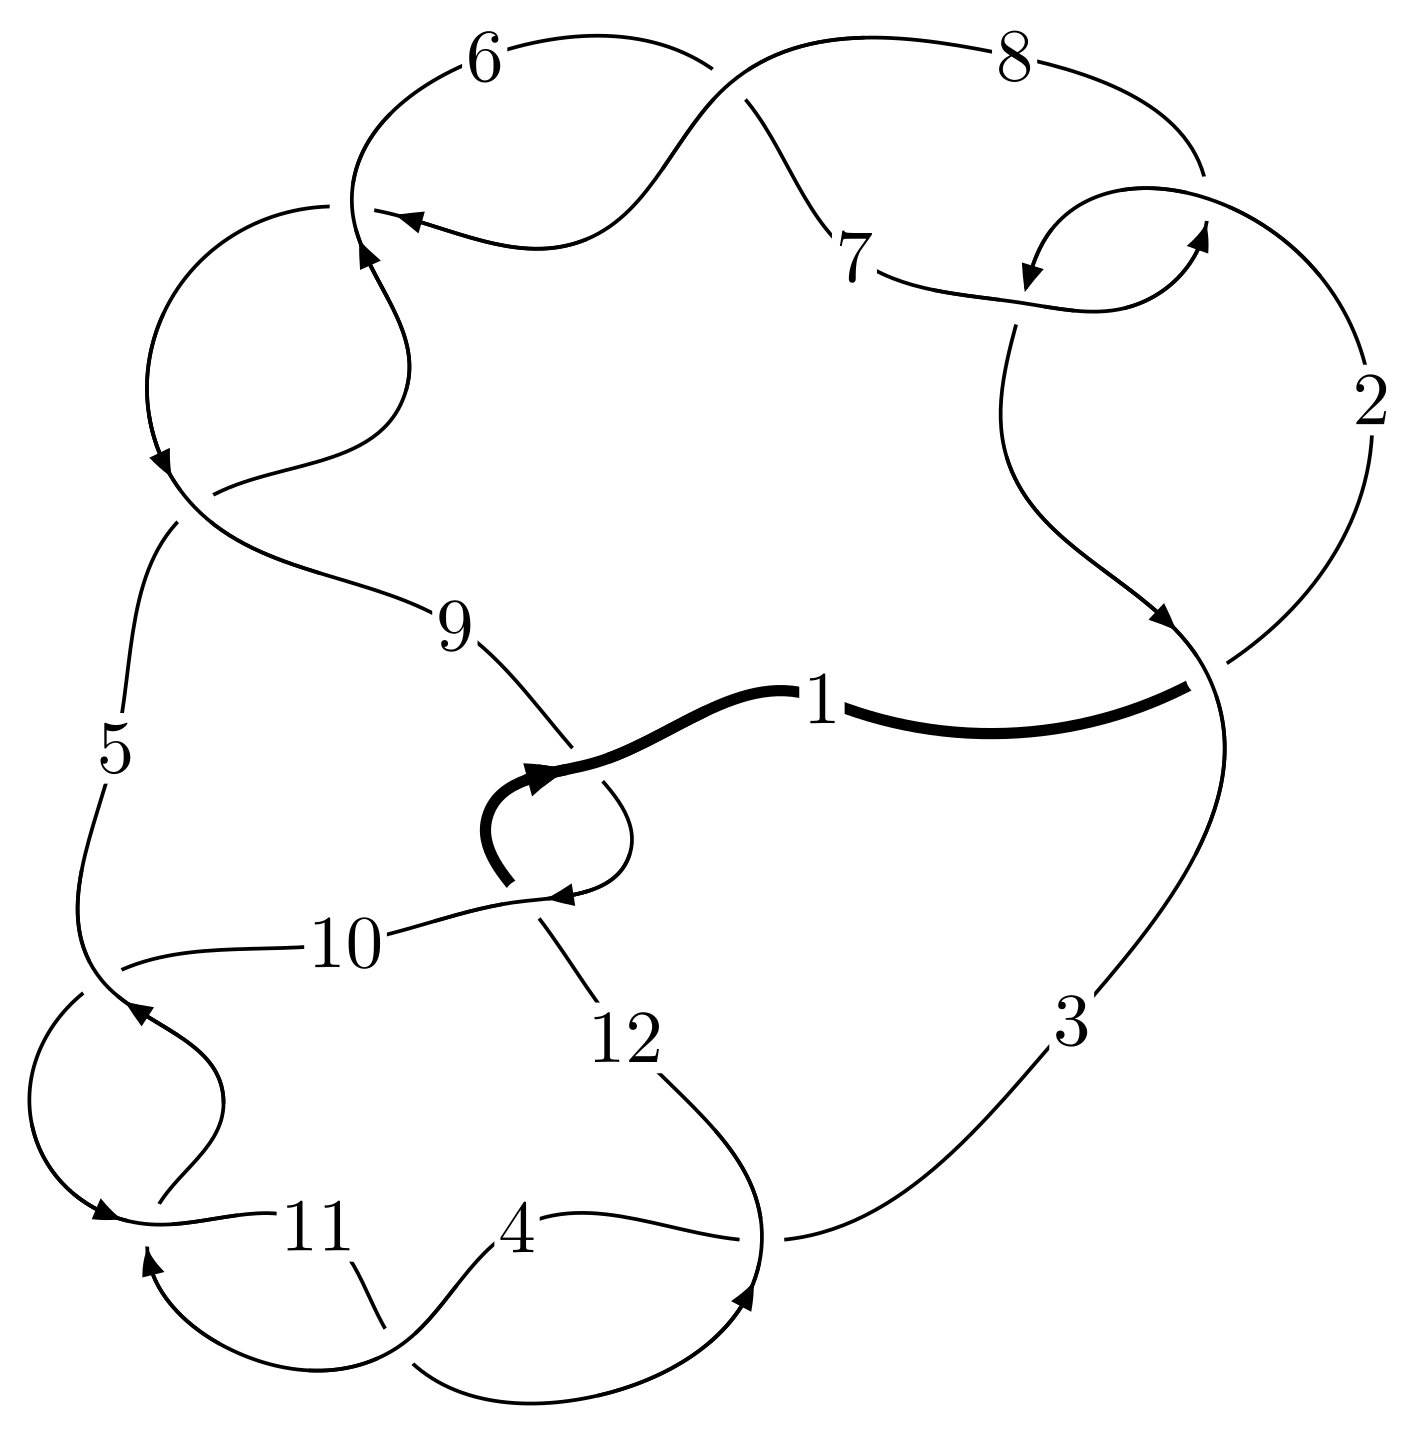
\includegraphics[width=112pt]{../../../GIT/diagram.site/Diagrams/png/1491_12a_0690.png}\\
\ \ \ A knot diagram\footnotemark}&
\allowdisplaybreaks
\textbf{Linearized knot diagam} \\
\cline{2-2}
 &
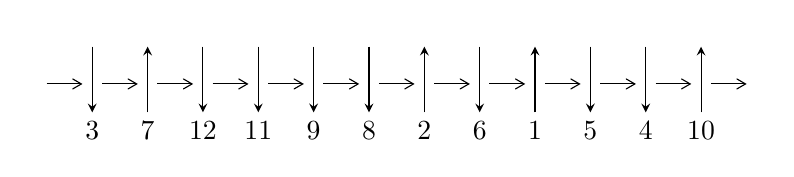
\begin{tikzpicture}[x=20pt, y=17pt]
	% nodes
	\node (C0) at (0, 0) {};
	\node (C1) at (1, 0) {};
	\node (C1U) at (1, +1) {};
	\node (C1D) at (1, -1) {3};

	\node (C2) at (2, 0) {};
	\node (C2U) at (2, +1) {};
	\node (C2D) at (2, -1) {7};

	\node (C3) at (3, 0) {};
	\node (C3U) at (3, +1) {};
	\node (C3D) at (3, -1) {12};

	\node (C4) at (4, 0) {};
	\node (C4U) at (4, +1) {};
	\node (C4D) at (4, -1) {11};

	\node (C5) at (5, 0) {};
	\node (C5U) at (5, +1) {};
	\node (C5D) at (5, -1) {9};

	\node (C6) at (6, 0) {};
	\node (C6U) at (6, +1) {};
	\node (C6D) at (6, -1) {8};

	\node (C7) at (7, 0) {};
	\node (C7U) at (7, +1) {};
	\node (C7D) at (7, -1) {2};

	\node (C8) at (8, 0) {};
	\node (C8U) at (8, +1) {};
	\node (C8D) at (8, -1) {6};

	\node (C9) at (9, 0) {};
	\node (C9U) at (9, +1) {};
	\node (C9D) at (9, -1) {1};

	\node (C10) at (10, 0) {};
	\node (C10U) at (10, +1) {};
	\node (C10D) at (10, -1) {5};

	\node (C11) at (11, 0) {};
	\node (C11U) at (11, +1) {};
	\node (C11D) at (11, -1) {4};

	\node (C12) at (12, 0) {};
	\node (C12U) at (12, +1) {};
	\node (C12D) at (12, -1) {10};
	\node (C13) at (13, 0) {};

	% arrows
	\draw[->,>={angle 60}]
	(C0) edge (C1) (C1) edge (C2) (C2) edge (C3) (C3) edge (C4) (C4) edge (C5) (C5) edge (C6) (C6) edge (C7) (C7) edge (C8) (C8) edge (C9) (C9) edge (C10) (C10) edge (C11) (C11) edge (C12) (C12) edge (C13) ;	\draw[->,>=stealth]
	(C1U) edge (C1D) (C2D) edge (C2U) (C3U) edge (C3D) (C4U) edge (C4D) (C5U) edge (C5D) (C6U) edge (C6D) (C7D) edge (C7U) (C8U) edge (C8D) (C9D) edge (C9U) (C10U) edge (C10D) (C11U) edge (C11D) (C12D) edge (C12U) ;
	\end{tikzpicture} \\
\hhline{~~} \\& 
\textbf{Solving Sequence} \\ \cline{2-2} 
 &
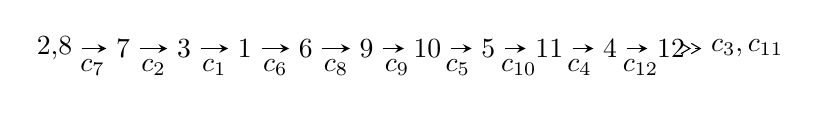
\begin{tikzpicture}[x=22pt, y=7pt]
	% node
	\node (A0) at (-1/8, 0) {2,8};
	\node (A1) at (1, 0) {7};
	\node (A2) at (2, 0) {3};
	\node (A3) at (3, 0) {1};
	\node (A4) at (4, 0) {6};
	\node (A5) at (5, 0) {9};
	\node (A6) at (6, 0) {10};
	\node (A7) at (7, 0) {5};
	\node (A8) at (8, 0) {11};
	\node (A9) at (9, 0) {4};
	\node (A10) at (10, 0) {12};
	\node (C1) at (1/2, -1) {$c_{7}$};
	\node (C2) at (3/2, -1) {$c_{2}$};
	\node (C3) at (5/2, -1) {$c_{1}$};
	\node (C4) at (7/2, -1) {$c_{6}$};
	\node (C5) at (9/2, -1) {$c_{8}$};
	\node (C6) at (11/2, -1) {$c_{9}$};
	\node (C7) at (13/2, -1) {$c_{5}$};
	\node (C8) at (15/2, -1) {$c_{10}$};
	\node (C9) at (17/2, -1) {$c_{4}$};
	\node (C10) at (19/2, -1) {$c_{12}$};
	\node (A11) at (45/4, 0) {$c_{3},c_{11}$};

	% edge
	\draw[->,>=stealth]	
	(A0) edge (A1) (A1) edge (A2) (A2) edge (A3) (A3) edge (A4) (A4) edge (A5) (A5) edge (A6) (A6) edge (A7) (A7) edge (A8) (A8) edge (A9) (A9) edge (A10) ;
	\draw[->>,>={angle 60}]	
	(A10) edge (A11);
\end{tikzpicture} \\ 

\end{tabular} \\

\footnotetext{
The image of knot diagram is generated by the software ``\textbf{Draw programme}" developed by Andrew Bartholomew(\url{http://www.layer8.co.uk/maths/draw/index.htm\#Running-draw}), where we modified some parts for our purpose(\url{https://github.com/CATsTAILs/LinksPainter}).
}\phantom \\ \newline 
\centering \textbf{Ideals for irreducible components\footnotemark of $X_{\text{par}}$} 
 
\begin{align*}
I^u_{1}&=\langle 
u^{44}+u^{43}+\cdots+3 u^2+1\rangle \\
\\
\end{align*}
\raggedright * 1 irreducible components of $\dim_{\mathbb{C}}=0$, with total 44 representations.\\
\footnotetext{All coefficients of polynomials are rational numbers. But the coefficients are sometimes approximated in decimal forms when there is not enough margin.}
\newpage
\renewcommand{\arraystretch}{1}
\centering \section*{I. $I^u_{1}= \langle u^{44}+u^{43}+\cdots+3 u^2+1 \rangle$}
\flushleft \textbf{(i) Arc colorings}\\
\begin{tabular}{m{7pt} m{180pt} m{7pt} m{180pt} }
\flushright $a_{2}=$&$\begin{pmatrix}0\\u\end{pmatrix}$ \\
\flushright $a_{8}=$&$\begin{pmatrix}1\\0\end{pmatrix}$ \\
\flushright $a_{7}=$&$\begin{pmatrix}1\\u^2\end{pmatrix}$ \\
\flushright $a_{3}=$&$\begin{pmatrix}u\\u^3+u\end{pmatrix}$ \\
\flushright $a_{1}=$&$\begin{pmatrix}u^3\\u^5+u^3+u\end{pmatrix}$ \\
\flushright $a_{6}=$&$\begin{pmatrix}u^2+1\\u^2\end{pmatrix}$ \\
\flushright $a_{9}=$&$\begin{pmatrix}u^4+u^2+1\\u^4\end{pmatrix}$ \\
\flushright $a_{10}=$&$\begin{pmatrix}- u^{12}- u^{10}-3 u^8-2 u^6+u^2+1\\- u^{14}-2 u^{12}-5 u^{10}-6 u^8-6 u^6-2 u^4- u^2\end{pmatrix}$ \\
\flushright $a_{5}=$&$\begin{pmatrix}u^6+u^4+2 u^2+1\\u^6+u^2\end{pmatrix}$ \\
\flushright $a_{11}=$&$\begin{pmatrix}u^{26}+3 u^{24}+\cdots+3 u^2+1\\u^{26}+2 u^{24}+\cdots- u^6- u^2\end{pmatrix}$ \\
\flushright $a_{4}=$&$\begin{pmatrix}u^{41}+4 u^{39}+\cdots-2 u^3+u\\u^{43}+5 u^{41}+\cdots+3 u^3+u\end{pmatrix}$ \\
\flushright $a_{12}=$&$\begin{pmatrix}u^{21}+2 u^{19}+7 u^{17}+10 u^{15}+14 u^{13}+12 u^{11}+5 u^9-2 u^7-5 u^5-2 u^3- u\\u^{23}+3 u^{21}+\cdots+2 u^3+u\end{pmatrix}$\\&\end{tabular}
\flushleft \textbf{(ii) Obstruction class $= -1$}\\~\\
\flushleft \textbf{(iii) Cusp Shapes $= -4 u^{42}-4 u^{41}+\cdots-12 u-6$}\\~\\
\newpage\renewcommand{\arraystretch}{1}
\flushleft \textbf{(iv) u-Polynomials at the component}\newline \\
\begin{tabular}{m{50pt}|m{274pt}}
Crossings & \hspace{64pt}u-Polynomials at each crossing \\
\hline $$\begin{aligned}c_{1},c_{5},c_{6}\\c_{8}\end{aligned}$$&$\begin{aligned}
&u^{44}+9 u^{43}+\cdots+6 u+1
\end{aligned}$\\
\hline $$\begin{aligned}c_{2},c_{7}\end{aligned}$$&$\begin{aligned}
&u^{44}+u^{43}+\cdots+3 u^2+1
\end{aligned}$\\
\hline $$\begin{aligned}c_{3},c_{4},c_{10}\\c_{11}\end{aligned}$$&$\begin{aligned}
&u^{44}- u^{43}+\cdots+2 u+1
\end{aligned}$\\
\hline $$\begin{aligned}c_{9},c_{12}\end{aligned}$$&$\begin{aligned}
&u^{44}+9 u^{43}+\cdots-8 u+1
\end{aligned}$\\
\hline
\end{tabular}\\~\\
\newpage\renewcommand{\arraystretch}{1}
\flushleft \textbf{(v) Riley Polynomials at the component}\newline \\
\begin{tabular}{m{50pt}|m{274pt}}
Crossings & \hspace{64pt}Riley Polynomials at each crossing \\
\hline $$\begin{aligned}c_{1},c_{5},c_{6}\\c_{8}\end{aligned}$$&$\begin{aligned}
&y^{44}+53 y^{43}+\cdots+38 y+1
\end{aligned}$\\
\hline $$\begin{aligned}c_{2},c_{7}\end{aligned}$$&$\begin{aligned}
&y^{44}+9 y^{43}+\cdots+6 y+1
\end{aligned}$\\
\hline $$\begin{aligned}c_{3},c_{4},c_{10}\\c_{11}\end{aligned}$$&$\begin{aligned}
&y^{44}+49 y^{43}+\cdots+6 y+1
\end{aligned}$\\
\hline $$\begin{aligned}c_{9},c_{12}\end{aligned}$$&$\begin{aligned}
&y^{44}+17 y^{43}+\cdots-10 y+1
\end{aligned}$\\
\hline
\end{tabular}\\~\\
\newpage\flushleft \textbf{(vi) Complex Volumes and Cusp Shapes}
$$\begin{array}{c|c|c}  
\text{Solutions to }I^u_{1}& \I (\text{vol} + \sqrt{-1}CS) & \text{Cusp shape}\\
 \hline 
\begin{aligned}
u &= \phantom{-}0.655099 + 0.751397 I\end{aligned}
 & \phantom{-}10.47210 + 2.42057 I & \phantom{-}5.00512 - 3.50428 I \\ \hline\begin{aligned}
u &= \phantom{-}0.655099 - 0.751397 I\end{aligned}
 & \phantom{-}10.47210 - 2.42057 I & \phantom{-}5.00512 + 3.50428 I \\ \hline\begin{aligned}
u &= \phantom{-}0.457290 + 0.880807 I\end{aligned}
 & -1.50378 + 2.68816 I & -5.95162 - 3.22752 I \\ \hline\begin{aligned}
u &= \phantom{-}0.457290 - 0.880807 I\end{aligned}
 & -1.50378 - 2.68816 I & -5.95162 + 3.22752 I \\ \hline\begin{aligned}
u &= -0.495314 + 0.905747 I\end{aligned}
 & -0.91674 - 6.42453 I & -3.67057 + 9.87108 I \\ \hline\begin{aligned}
u &= -0.495314 - 0.905747 I\end{aligned}
 & -0.91674 + 6.42453 I & -3.67057 - 9.87108 I \\ \hline\begin{aligned}
u &= -0.379628 + 0.881690 I\end{aligned}
 & \phantom{-}4.48646 - 0.62493 I & -2.71495 + 3.55329 I \\ \hline\begin{aligned}
u &= -0.379628 - 0.881690 I\end{aligned}
 & \phantom{-}4.48646 + 0.62493 I & -2.71495 - 3.55329 I \\ \hline\begin{aligned}
u &= \phantom{-}0.520660 + 0.926121 I\end{aligned}
 & \phantom{-}6.20074 + 8.92581 I & -0.06506 - 8.28337 I \\ \hline\begin{aligned}
u &= \phantom{-}0.520660 - 0.926121 I\end{aligned}
 & \phantom{-}6.20074 - 8.92581 I & -0.06506 + 8.28337 I \\ \hline\begin{aligned}
u &= -0.075736 + 0.916828 I\end{aligned}
 & \phantom{-}2.88611 - 4.18901 I & -5.84139 + 3.97616 I \\ \hline\begin{aligned}
u &= -0.075736 - 0.916828 I\end{aligned}
 & \phantom{-}2.88611 + 4.18901 I & -5.84139 - 3.97616 I \\ \hline\begin{aligned}
u &= -0.558233 + 0.724774 I\end{aligned}
 & \phantom{-}2.78376 - 2.11026 I & \phantom{-}4.66535 + 4.95546 I \\ \hline\begin{aligned}
u &= -0.558233 - 0.724774 I\end{aligned}
 & \phantom{-}2.78376 + 2.11026 I & \phantom{-}4.66535 - 4.95546 I \\ \hline\begin{aligned}
u &= \phantom{-}0.027533 + 0.895789 I\end{aligned}
 & -3.76094 + 1.84552 I & -10.24133 - 4.26971 I \\ \hline\begin{aligned}
u &= \phantom{-}0.027533 - 0.895789 I\end{aligned}
 & -3.76094 - 1.84552 I & -10.24133 + 4.26971 I \\ \hline\begin{aligned}
u &= \phantom{-}0.672800 + 0.488934 I\end{aligned}
 & \phantom{-}7.59840 - 4.48618 I & \phantom{-}3.71469 + 2.30966 I \\ \hline\begin{aligned}
u &= \phantom{-}0.672800 - 0.488934 I\end{aligned}
 & \phantom{-}7.59840 + 4.48618 I & \phantom{-}3.71469 - 2.30966 I \\ \hline\begin{aligned}
u &= -0.608827 + 0.473439 I\end{aligned}
 & \phantom{-}0.43015 + 2.25708 I & \phantom{-}0.48990 - 3.95946 I \\ \hline\begin{aligned}
u &= -0.608827 - 0.473439 I\end{aligned}
 & \phantom{-}0.43015 - 2.25708 I & \phantom{-}0.48990 + 3.95946 I \\ \hline\begin{aligned}
u &= \phantom{-}0.855723 + 0.916416 I\end{aligned}
 & \phantom{-}11.73180 + 3.17974 I & \phantom{-}1.84300 - 2.50377 I \\ \hline\begin{aligned}
u &= \phantom{-}0.855723 - 0.916416 I\end{aligned}
 & \phantom{-}11.73180 - 3.17974 I & \phantom{-}1.84300 + 2.50377 I \\ \hline\begin{aligned}
u &= -0.888935 + 0.892951 I\end{aligned}
 & \phantom{-}6.98756 - 1.09197 I & -1.86937 + 2.51379 I \\ \hline\begin{aligned}
u &= -0.888935 - 0.892951 I\end{aligned}
 & \phantom{-}6.98756 + 1.09197 I & -1.86937 - 2.51379 I \\ \hline\begin{aligned}
u &= \phantom{-}0.902652 + 0.887567 I\end{aligned}
 & \phantom{-}8.07252 - 2.80136 I & \phantom{-0.000000 -}0. + 3.37397 I \\ \hline\begin{aligned}
u &= \phantom{-}0.902652 - 0.887567 I\end{aligned}
 & \phantom{-}8.07252 + 2.80136 I & \phantom{-0.000000 } 0. - 3.37397 I \\ \hline\begin{aligned}
u &= -0.913567 + 0.886340 I\end{aligned}
 & \phantom{-}15.5582 + 5.3967 I & \phantom{-}3.71419 - 2.08485 I \\ \hline\begin{aligned}
u &= -0.913567 - 0.886340 I\end{aligned}
 & \phantom{-}15.5582 - 5.3967 I & \phantom{-}3.71419 + 2.08485 I \\ \hline\begin{aligned}
u &= \phantom{-}0.885790 + 0.925568 I\end{aligned}
 & \phantom{-}11.28050 + 3.27174 I & \phantom{-}4.41927 - 2.54057 I \\ \hline\begin{aligned}
u &= \phantom{-}0.885790 - 0.925568 I\end{aligned}
 & \phantom{-}11.28050 - 3.27174 I & \phantom{-}4.41927 + 2.54057 I\\
 \hline 
 \end{array}$$\newpage$$\begin{array}{c|c|c}  
\text{Solutions to }I^u_{1}& \I (\text{vol} + \sqrt{-1}CS) & \text{Cusp shape}\\
 \hline 
\begin{aligned}
u &= -0.864280 + 0.949514 I\end{aligned}
 & \phantom{-}6.80746 - 5.39327 I & -2.17460 + 2.29017 I \\ \hline\begin{aligned}
u &= -0.864280 - 0.949514 I\end{aligned}
 & \phantom{-}6.80746 + 5.39327 I & -2.17460 - 2.29017 I \\ \hline\begin{aligned}
u &= \phantom{-}0.868528 + 0.961101 I\end{aligned}
 & \phantom{-}7.83679 + 9.34211 I & \phantom{-0.000000 } 0. - 8.07187 I \\ \hline\begin{aligned}
u &= \phantom{-}0.868528 - 0.961101 I\end{aligned}
 & \phantom{-}7.83679 - 9.34211 I & \phantom{-0.000000 -}0. + 8.07187 I \\ \hline\begin{aligned}
u &= -0.903374 + 0.934414 I\end{aligned}
 & -19.6382 - 3.3289 I & \phantom{-}5.91897 + 2.37042 I \\ \hline\begin{aligned}
u &= -0.903374 - 0.934414 I\end{aligned}
 & -19.6382 + 3.3289 I & \phantom{-}5.91897 - 2.37042 I \\ \hline\begin{aligned}
u &= -0.873373 + 0.968938 I\end{aligned}
 & \phantom{-}15.2918 - 11.9872 I & \phantom{-}3.20276 + 6.75389 I \\ \hline\begin{aligned}
u &= -0.873373 - 0.968938 I\end{aligned}
 & \phantom{-}15.2918 + 11.9872 I & \phantom{-}3.20276 - 6.75389 I \\ \hline\begin{aligned}
u &= \phantom{-}0.326627 + 0.532554 I\end{aligned}
 & -0.166341 + 0.920466 I & -3.92535 - 6.51014 I \\ \hline\begin{aligned}
u &= \phantom{-}0.326627 - 0.532554 I\end{aligned}
 & -0.166341 - 0.920466 I & -3.92535 + 6.51014 I \\ \hline\begin{aligned}
u &= -0.558336 + 0.208664 I\end{aligned}
 & \phantom{-}6.42918 - 2.63981 I & \phantom{-}3.65305 + 2.69802 I \\ \hline\begin{aligned}
u &= -0.558336 - 0.208664 I\end{aligned}
 & \phantom{-}6.42918 + 2.63981 I & \phantom{-}3.65305 - 2.69802 I \\ \hline\begin{aligned}
u &= \phantom{-}0.446901 + 0.368826 I\end{aligned}
 & -0.171380 + 0.972064 I & -1.26603 - 5.13929 I \\ \hline\begin{aligned}
u &= \phantom{-}0.446901 - 0.368826 I\end{aligned}
 & -0.171380 - 0.972064 I & -1.26603 + 5.13929 I\\
 \hline 
 \end{array}$$\newpage
\newpage\renewcommand{\arraystretch}{1}
\centering \section*{ II. u-Polynomials}
\begin{tabular}{m{50pt}|m{274pt}}
Crossings & \hspace{64pt}u-Polynomials at each crossing \\
\hline $$\begin{aligned}c_{1},c_{5},c_{6}\\c_{8}\end{aligned}$$&$\begin{aligned}
&u^{44}+9 u^{43}+\cdots+6 u+1
\end{aligned}$\\
\hline $$\begin{aligned}c_{2},c_{7}\end{aligned}$$&$\begin{aligned}
&u^{44}+u^{43}+\cdots+3 u^2+1
\end{aligned}$\\
\hline $$\begin{aligned}c_{3},c_{4},c_{10}\\c_{11}\end{aligned}$$&$\begin{aligned}
&u^{44}- u^{43}+\cdots+2 u+1
\end{aligned}$\\
\hline $$\begin{aligned}c_{9},c_{12}\end{aligned}$$&$\begin{aligned}
&u^{44}+9 u^{43}+\cdots-8 u+1
\end{aligned}$\\
\hline
\end{tabular}\newpage\renewcommand{\arraystretch}{1}
\centering \section*{ III. Riley Polynomials}
\begin{tabular}{m{50pt}|m{274pt}}
Crossings & \hspace{64pt}Riley Polynomials at each crossing \\
\hline $$\begin{aligned}c_{1},c_{5},c_{6}\\c_{8}\end{aligned}$$&$\begin{aligned}
&y^{44}+53 y^{43}+\cdots+38 y+1
\end{aligned}$\\
\hline $$\begin{aligned}c_{2},c_{7}\end{aligned}$$&$\begin{aligned}
&y^{44}+9 y^{43}+\cdots+6 y+1
\end{aligned}$\\
\hline $$\begin{aligned}c_{3},c_{4},c_{10}\\c_{11}\end{aligned}$$&$\begin{aligned}
&y^{44}+49 y^{43}+\cdots+6 y+1
\end{aligned}$\\
\hline $$\begin{aligned}c_{9},c_{12}\end{aligned}$$&$\begin{aligned}
&y^{44}+17 y^{43}+\cdots-10 y+1
\end{aligned}$\\
\hline
\end{tabular}
\vskip 2pc
\end{document}